\section{Experiment}\label{sec:experiment}
We recorded the frame per second (FPS) experiment\footnote{https://github.com/ZJUVAG/NetV.js/tree/benchmarks/benchmarks} to test the rendering performance of \name with other popular tools and libraries which are supports graph rendering, including D3-SVG, D3-Canvas, Cytoscape.js, Sigma.js, and Stardust.js. In particular, \name, Sigma.js, and Stardust.js use WebGL to render data. To simulate real-world graph data, we set the graph density as 20, which means the ratio of the number of edges to the number of nodes is 1 to 20. The display refresh rate is 144Hz; the GPU is GTX 1060 with 6G.


It is shown that \autoref{fig:eva}, \name, Stardust.js, and D3-Canvas can render around 100 thousand elements. \name can render more than 1 million elements with FPS greater than 1.

\begin{figure}[htbp]
    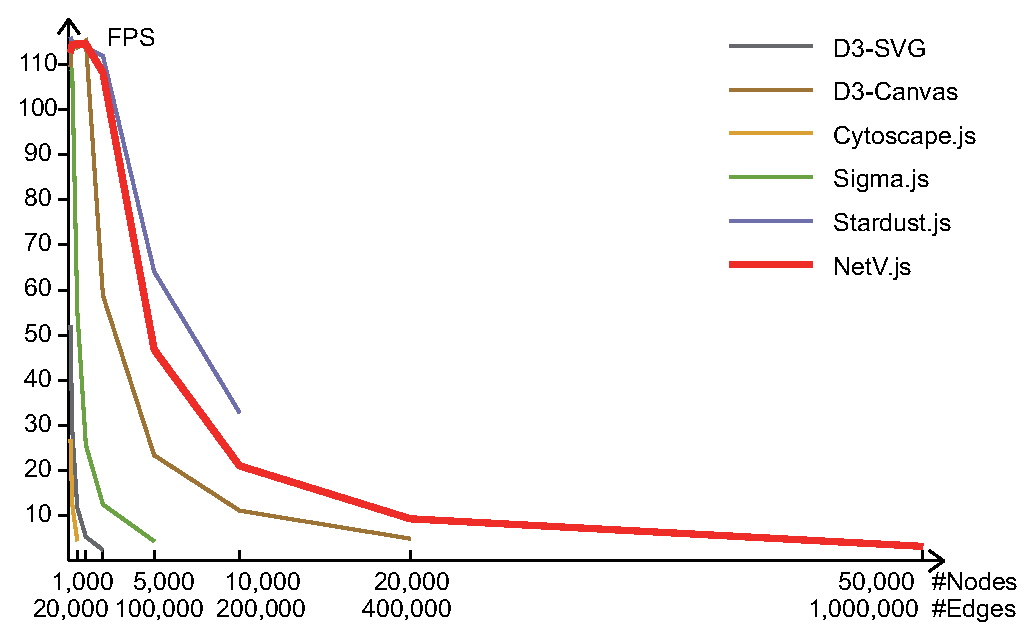
\includegraphics[width=\linewidth]{fig/eva.eps}
    \caption{
        Performance comparison among 6 toolkits.
    }
    \label{fig:eva}
\end{figure}
